% Suppress warnings about PDF version
\pdfminorversion=7
\documentclass[final,USenglish,colophon]{phduio}
\usepackage{pdfpages}
\usepackage{phdstyle}
\usepackage[toc,acronym,seeautonumberlist,nohypertypes={nolist},nopostdot]{glossaries}
\usepackage{glossaries-extra}
\usepackage{xparse,xstring}
\usepackage{subcaption}
\usepackage[all]{hypcap}
\usepackage{thm-restate}
%\usepackage{layout}
%\usepackage{showframe}

% See the following links for documentation:
% https://www.mn.uio.no/english/research/phd/thesis-adjudication/layout/latex-template.html
% https://github.com/uio-latex/phduio-article-based
% https://github.com/uio-latex/phduio-monograph
%
% https://www.mn.uio.no/ifi/tjenester/it/hjelp/latex/biblatex-guide.pdf
% https://ctan.uib.no/macros/latex/contrib/biblatex/doc/biblatex.pdf


\author{Jonas S{\ae}ther Markussen}
\title{SmartIO: Device sharing and memory disaggregation in PCIe clusters using non-transparent bridging}

\department{Department of Informatics}
\faculty{Faculty of Mathematics and Natural Sciences}

% Additional affiliations
\affiliation{
    Dolphin Interconnect Solutions
    \AND
    Simula Research Laboratory
}

% Request correct numbers from repro@uio.no
\ISSN{xxxx-xxxx}
\dissertationseries{xxxx}


% Make cleveref say "page" instead of "Page"
\AtBeginDocument{%
    \crefname{page}{page}{pages}%
}


% Include article
\DeclareDocumentCommand{\includepaper}{ O{} O{} m m}{
	% We don't want to prefix section titles with the chapter number in the TOC for the papers
	\counterwithout{section}{chapter}
	\setcounter{section}{0}

    \label{#3}
    \includearticle[#1]{papers/#3}{#4}

	% Restore section titles prefix the chapter number
	\counterwithin{section}{chapter}

    % Add two blank pages after paper
    \ifthenelse{\equal{#2}{}}{%
        \newpage\thispagestyle{empty}~\newpage\thispagestyle{empty}%
    }{%
        \newpage\thispagestyle{empty}
    }
}


% Can't ever have enough headlines in TOC
\setcounter{secnumdepth}{3}
\setcounter{tocdepth}{3}



% Referring to sections in the papers from the main body of the dissertation
\NewDocumentCommand{\getpaper}{m m}{#1}
\NewDocumentCommand{\getsect}{m m}{#1:#2}

\NewDocumentCommand{\papersectpageref}{m}{~(on~\cpageref{#1})}

\NewDocumentCommand{\makepapersectref}
{ m m }
{%
    \IfStrEq{#2}{NOSECT}%
    {%
        \cref{#1}\papersectpageref{#1}%
    }%
    {%
        \StrCount{#2}{,}[\papersectrefcount]%
        \ifthenelse{\equal{\papersectrefcount}{0}}%
        {\hyperref[#2]{\cref*{#2} of \cref*{#1}}\papersectpageref{#2}}%
        {\cref{#2} of \cref*{#1}\papersectpageref{#2}}%
    }%
}

\NewDocumentCommand{\addpapersectrefhelper}
{ m m }
{%
    \IfNoValueTF{#2}%
    {%
        \pgfkeyssetvalue{/{\getpaper{#1}{#2}}}{NOSECT}%
    }%
    {%
        \pgfkeysifdefined{/{\getpaper{#1}{#2}}}%
        {\pgfkeyssetevalue{/{\getpaper{#1}{#2}}}{\pgfkeysvalueof{/{\getpaper{#1}{#2}}},{\getsect{#1}{#2}}}}%
        {\pgfkeyssetvalue{/{\getpaper{#1}{#2}}}{\getsect{#1}{#2}}}%
    }%
}

\NewDocumentCommand{\addpapersectref}
{ > {\SplitArgument{1}{:}}m }
{%
    \addpapersectrefhelper #1%
%    \pgfkeysifdefined{/{\getpaper #1}}%
%    {\pgfkeyssetevalue{/{\getpaper #1}}{\pgfkeysvalueof{/{\getpaper #1}},{\getsect #1}}}%
%    {\pgfkeyssetvalue{/{\getpaper #1}}{\getsect #1}}%
}

\NewDocumentCommand{\makepapersectrefs}
{ > {\SplitArgument{1}{:}}m }
{%
    \pgfkeysifdefined{/{\getpaper #1}}
    {%
        \ifthenelse{\equal{\pgfkeysvalueof{/{\getpaper #1}}}{}}
        {%
        }%
        {%
            \paperrefand{}\makepapersectref{{\getpaper #1}}{\pgfkeysvalueof{/{\getpaper #1}}}%
            \renewcommand{\paperrefand}{ and }%
            \pgfkeyssetvalue{/{\getpaper #1}}{}%
        }%
    }%
    {}%
}

\NewDocumentCommand{\paperref}
{ > { \SplitList {,} } m }
{\begingroup\newcommand{\paperrefand}{}\ProcessList{#1}{\addpapersectref}\ProcessList{#1}{\makepapersectrefs}\endgroup}



% Research question and proposition/objectives/requirements
\makeatletter
\newenvironment{question}
{\begin{quote}\itshape}
{\end{quote}\ignorespacesafterend\noindent}
\makeatother

%\declaretheoremstyle[
%    name={Research Question},
%    headfont=\bfseries\sffamily,
%    notefont=\normalfont,
%    bodyfont=\normalfont\itshape,
%    headpunct={:},
%    spaceabove=\topsep,
%    spacebelow=\topsep,
%]{question}
%\declaretheorem[
%    style=question,
%    numbered=no,
%    preheadhook=\ignorespacesafterend,
%    postheadhook=\noindent\protect\leftskip=2em\rightskip=2em,
%    postfoothook=\ignorespacesafterend\noindent
%]{question}

\declaretheoremstyle[
    name={Objective},
    headfont=\bfseries\sffamily,
    notefont=\normalfont,
    bodyfont=\normalfont,
    headpunct={:},
    spaceabove=18pt,
    spacebelow=6pt,
    postheadhook=\protect\leftskip=0em\rightskip=0em\hangindent=2.6em,
    postfoothook=\ignorespacesafterend\noindent
]{objective}
\declaretheorem[
    style=objective,
    numbered=yes
]{objective}
\crefrangeformat{objective}{Objectives~#3#1#4--#5#2#6}
\Crefrangeformat{objective}{Objectives~#3#1#4--#5#2#6}
\crefname{objective}{Objective}{Objectives}
\Crefname{objective}{Objective}{Objectives}



% Glossary stuff
\newglossary[nolistg]{nolist}{nolists}{nolisto}{not listed}
\makeglossaries
\setabbreviationstyle[acronym]{long-short}
\def\myglossarytitle{Glossary}

\renewcommand{\glsseeformat}[3][\seename]{%
    \\*%
    \emph{#1} \glsseelist{#2}%
}

% Some terms have both an acronym and needs a glossary entry
\DeclareDocumentCommand{\newdualentry}{ O{} O{} m m m m }{
	\newglossaryentry{gls-#3}{
        name={#5 (#4)},
        sort={#5},
		description={#6},#1
	}
    \makeglossaries
    \newglossaryentry{#3}{
        type=\acronymtype,
        name={#4},
        see={[\myglossarytitle:]{gls-#3}},
        description={#5},%\glsseeformat[\myglossarytitle:]{gls-#3}{}},
        long={#5\glsadd{gls-#3}},
        longplural={#5s\glsadd{gls-#3}},
        text={#4\glsadd{gls-#3}},
        short={#4\glsadd{gls-#3}},
        shortplural={#4s\glsadd{gls-#3}},
        first={#5~(#4)\glsadd{gls-#3}},
        firstplural={#5s~(#4s)\glsadd{gls-#3}},#2
    }
    \newglossaryentry{nolist-#3}{
        name={#4},
        long={#5},
        type=nolist,
        description={#5},
        longplural={#5s},
        short={#4},
        shortplural={#4s},
        first={#4},
        firstplural={#5s},#2
    }
    \makeglossaries
}


% Get the display text of an abbreviation without linking in the glossary
% Use this to link to glossary entries from a glossary entry description, 
% without adding to the numbers list.
\DeclareDocumentCommand{\glsabbrlink}{ m }{%
    \ifglsentryexists{nolist-#1}{%
        \glshyperlink[\glsfmtshort{nolist-#1}]{gls-#1}%
    }{%
        \glshyperlink[\glsfmtshort{#1}]{#1}%
    }%
}
\DeclareDocumentCommand{\glsabbrlinkpl}{ m }{%
    \ifglsentryexists{nolist-#1}{%
        \glshyperlink[\glsfmtshortpl{nolist-#1}]{gls-#1}%
    }{%
        \glshyperlink[\glsfmtshortpl{#1}]{#1}%
    }%
}
\DeclareDocumentCommand{\glsglossarylink}{ m }{%
    \ifglsentryexists{nolist-#1}{%
        \glshyperlink[\glsentrytext{nolist-#1}]{gls-#1}%
    }{%
        \glshyperlink[\glsentrytext{#1}]{#1}%
    }%
}


% Some terms need to refer something else in the glossary
\DeclareDocumentCommand{\newlinkedacronym}{ O{} m m m m }{
    \newacronym[
        see={[\myglossarytitle:]{#2}},
        first={#5~(#4)\glsadd{#2}},
        firstplural={#5s~(#4s)\glsadd{#2}},
        short={#4\glsadd{#2}},
        shortplural={#4s\glsadd{#2}},
        long={#5\glsadd{#2}},
        longplural={#5s\glsadd{#2}},#1
    ]{#3}{#4}{#5}
    \makeglossaries
}

% Link to a glossary entry while using a custom text
\DeclareDocumentCommand{\lgls}{ m m }{\glsdisp{#1}{#2}\glsadd{#1}\ifglsentryexists{gls-#1}{\glsadd{gls-#1}}{}}

% Define a custom text and link it to a glossary entry
\DeclareDocumentCommand{\linkedgls}{ m m m }{%
    \newglossaryentry{linked-#2}{
        name={#2},
        description={#2},
        text={#3},
        type=nolist
    }
    \makeglossaries
    \pgfkeyssetvalue{/glskey/#2}{#1}%
}

% Glossaries hack
\let\origgls\gls
\renewcommand{\gls}[1]{%
    \pgfkeysifdefined{/glskey/#1}{%
        \lgls{\pgfkeysvalueof{/glskey/#1}}{\glsentrytext{linked-#1}}%
    }{%
        \origgls{#1}%
    }%
}
\let\origGls\Gls
\renewcommand{\Gls}[1]{%
    \pgfkeysifdefined{/glskey/#1}{%
        \lgls{\pgfkeysvalueof{/glskey/#1}}{\Glsentrytext{linked-#1}}%
    }{%
        \origGls{#1}%
    }%
}
\let\origglspl\glspl
\renewcommand{\glspl}[1]{%
    \pgfkeysifdefined{/glskey/#1}{%
        \lgls{\pgfkeysvalueof{/glskey/#1}}{\glsentryplural{linked-#1}}%
    }{%
        \origglspl{#1}%
    }%
}
\let\origGlspl\Glspl
\renewcommand{\Glspl}[1]{%
    \pgfkeysifdefined{/glskey/#1}{%
        \lgls{\pgfkeysvalueof{/glskey/#1}}{\Glsentryplural{linked-#1}}%
    }{%
        \origGlspl{#1}%
    }%
}


% Include glossary definitions
\makeglossaries

% Some basic computer related abbreviations not necessary to define for first use
\newacronym{bios}{BIOS}{Basic Input/Output System}
\glsunset{bios}

\newdualentry{io}{I/O}{input/output}
{Any interaction with a hardware device}
\glsunset{io}

\newacronym{ram}{RAM}{random access memory}

\newacronym{cpu}{CPU}{central processing unit}

\newacronym[plural={OSes}]{os}{OS}{operating system}

\newacronym{pci}{PCI}{Peripheral Component Interconnect}
\newacronym{pcie}{PCIe}{Peripheral Component Interconnect Express}


\newacronym{nvme}{NVMe}{non-volatile memory express storage device}
\newacronym{nvmeof}{NVMe-oF}{NVMe over Fabrics}
\newacronym{ssd}{SSD}{solid-state flash memory storage device}
\newacronym{gpu}{GPU}{graphics processing unit}
\newacronym{fpga}{FPGA}{field-programmable gate array}
\newacronym{nic}{NIC}{network interface card}
\newacronym{pf}{PF}{physical device function}
\newacronym{mriov}{MR-IOV}{Multi-Root I/O Virtualization}
\newacronym{api}{API}{application programming interface}
\newacronym{msi}{MSI}{message-signalled interrupts}
\newacronym{msix}{MSI-X}{extended message-signalled interrupts}
\newacronym{vm}{VM}{virtual machine}
\newacronym{mdev}{MDEV}{Mediated Device Driver}
\newacronym{sisci}{SISCI}{Software Infrastructure Shared-Memory Cluster Interconnect}
\newacronym{fio}{FIO}{Flexible I/O tester}


\newdualentry{sriov}{SR-IOV}{Single-Root I/O Virtualization}
{Allows a single device to virtualize multiple device functions in hardware}

\newdualentry{dma}{DMA}{direct memory access}
{Devices capable of direct memory access can access system memory and even memory regions of other devices}

\newdualentry{rdma}{RDMA}{remote direct memory access}
{Using the network adapter to copy memory directly onto the network, without going through the network stack}

\newdualentry{ntb}{NTB}{non-transparent bridge}
{A special \glsfmtshort{pcie} device that translates memory transactions between different address domains}

\newdualentry{bar}{BAR}{Base Address Register}
{The start address of a memory region of a device, used synonymously for the device memory region itself}

\newglossaryentry{p2p}{
    name={peer-to-peer},
    description={A \glsfmtshort{pcie} feature allowing two devices to directly transfer data between each other without going through host \glsfmtshort{ram}}
}

\newglossaryentry{disaggregation}{
	name={disaggregation},
	description={Dividing up a resource, such as memory or a device, into smaller components, and making them available to remote units}
}

\newglossaryentry{kernel space}{
    name={kernel space},
    description={Virtual memory and execution privileges suitable for \glsfmtlong{os} kernel and device drivers}
}

\newglossaryentry{userspace}{
    name={user space},
    description={Virtual memory and execution privileges suitable for application software, in contrast to kernel space}
}

\newglossaryentry{passthrough}{
    name={pass-through},
    description={Allowing a physical hardware device to be accessed directly by a \glsfmtlong{vm} guest by using a system's \glsfmtlong{iommu} to map memory for the device}
}

\newglossaryentry{guest}{
    name={virtual machine guest},
    description={A software-emulated computer system},
    text={guest}
}

\newglossaryentry{host}{
    name={virtual machine host},
    description={The physical machine running one or more \glsfmtlongpl{vm}},
    text={host}
}


\newglossaryentry{middleware}{
    name={middleware},
    description={A software service that provides facilitation beyond functionality available from the \glsfmtlong{os}}
}


\newglossaryentry{paravirtualization}{
	name={paravirtualization},
	description={A paravirtualized device relies on facilitation by the hypervisor in order to use host resources}
}

\newglossaryentry{hypervisor}{
	name={hypervisor},
	description={Kernel space software on a \glsfmtlong{vm} host, assisting and facilitating a virtual machine emulator (such as Qemu)}
}


\newdualentry{iommu}{IOMMU}{I/O Memory Management Unit}
{A unit embedded on the \glsfmtlong{cpu} that creates separate virtual address spaces for devices and prevents \glsfmtlong{dma} transactions outside these virtual address spaces}


\newlinkedacronym{hypervisor}{kvm}{KVM}{Linux kernel-based virtual machine hypervisor}

\newlinkedacronym{gls-sriov}{vf}{VF}{virtual device function}


\makeglossaries


\begin{document}
	% Folios in Roman numerals, unnumbered chapters.
	\frontmatter 

	\uiotitle

	% Do some hyperref magic because we don't like
	% the template defaults
	\hypersetup{
		hidelinks, % no borders around links
		%colorlinks=false, % don't color links
		linktoc=all, % link to pages in TOC as well
	}

	% Prefacing sections
	%\thispagestyle{empty}
\vspace*{\stretch{1}}
\begin{flushright}
\emph{Dedisert til mine venner --- alltid har dere v{\ae}rt der for meg.}
\end{flushright}
\vspace*{\stretch{3}}


	\chapter{Abstract}
%Remote resources can be accessed directly over native \gls{pcie}, without requiring any software in the critical path or network protocol translation.
%%
%SmartIO seamlessly combines traditional \gls{io} with distributed shared-memory functionality, and is able to provide sharing and disaggregation capabilities at multiple abstraction levels:
%distributing devices to physical hosts, distributing devices to \glspl{vm}, and enabling disaggregation of devices and memory resources in software.
%%
%Furthermore, by using \gls{pcie} shared memory techniques, SmartIO is able to abstract away the physical location of devices and memory resources. 
%Our implementation translates memory addresses between different address domains and resolves paths through the \gls{pcie} network in a manner that is transparent to application software, device drivers, and even the \gls{os}.

This unlocks a new potential in PCIe-connected cluster systems, as application software no longer needs to be written with accessing remote resources in mind, but can be implemented as if resources are local.
%without requiring

%minimize data movement

%allow all host to contribute their own/local resources
%abstract away resources, blur the distinction. unlock new potential, in a manner that is transparent
%unlocks a new potential (for abstract maybe?)

	\chapter{Preface}
TODO


\section*{Acknowledgements}

Thanks for all the fish!


\vskip\onelineskip
\begin{flushleft}
    \sffamily
    \uiocolon\textbf{\theauthor}
    \\
    Oslo,\MONTH\the\year
\end{flushleft}


	% Paper list
	\cleartorecto
	\chapter{List of papers}
	\section*{\cref{paper:nossdav}}
	\fullcite{paper:nossdav}
	\section*{\cref{paper:mmsys}}
	\fullcite{paper:mmsys}
	\section*{\cref{paper:srmpds}}
	\fullcite{paper:srmpds}
	\section*{\cref{paper:cc}}
	\fullcite{paper:cc}
	\section*{\cref{paper:tocs}}
	\fullcite{paper:tocs}

	% We don't like uppercase in section titles
	\renewcommand{\listfigurename}{List of figures}
	\renewcommand{\listtablename}{List of tables}

	% Print all of the other lists
	\cleartorecto
	\tableofcontents
	\cleartorecto
	\listoffigures
	%\cleartorecto
	%\listoftables
	\cleartorecto
	\setglossarystyle{list}
    \printglossary[title=List of abbreviations,type=\acronymtype]%,nonumberlist]

	% Folios in Arabic numerals, numbered chapters.
	\mainmatter

	\chapter{Introduction}\label{chapter:intro}
Modern cluster computing applications often have high requirements to \gls{io} performance.
%
For example, many computing clusters rely on compute accelerators, such as \glspl{gpu} and \glspl{fpga}, to increase the processing speed.
%
In recent years, we have also seen a convergence of the high-performance computing, big~data, and machine~learning research fields.
%
This has led to new demands to \gls{io} performance where distributed, high-volume storage is becoming a requirement for high-performance computing, while low latency networking and facilitating access to compute accelerators have become cloud computing issues~\cite{Trivedi2011,Coates2013,Taherkordi2018}.
%
If resources are distributed scarcely in the cluster, cluster machines with resources may become bottlenecks when a workload requires heavy computation on \glspl{gpu} or fast access to storage.
%
Contrarily, over-provisioning machines with resources may lead to devices becoming underutilized if the workload's demands are more sporadic.
%
Heterogeneous workloads may even require widely different compositions of devices and memory resources for individual machines.
%
Being able to share and dynamically partition devices between machines in a cluster leads to more efficient
utilization, as individual machines may scale up or down \gls{io} resources based on current workload requirements.



In cloud computing environments, such dynamic scaling and resource partitioning is often handled through virtualization. 
\Gls{vm} \glspl{hypervisor} may dynamically add virtual \gls{io} devices to \gls{vm} instances on demand.
%
It is even possible to temporarily suspend computation to migrate \glspl{vm} to \gls{host} machines with more hardware resources available, should the \gls{vm}'s requirements exceed the available local resources.
%
However, resource virtualization may not be viable when the raw, bare-metal \gls{io} performance is required, for example in the case of \gls{gpu}-intensive machine~learning workloads.
%
In this regard, it is possible to \glslink{passthrough}{``pass through''} physical \gls{io} devices to a \gls{vm} \gls{guest} using an \gls{iommu}.
%
The \gls{iommu} facilitates direct access to hardware from the \gls{guest} without compromising the virtualized environment.
%
Although \gls{passthrough} allows physical hardware to be used with minimal software overhead, this technique suffers from a lack of flexibility as the physical devices are tightly coupled with the hosts they are installed in.
%
Distributing VMs across hosts in the network in a way that maximizes resource utilization and adapts dynamically to varying gls{io} requirements, without sacrificing the bare-metal performance that pass-through provides, remains a challenge.



Another challenge is the networking technology itself. 
Despite having been a research topic for decades, moving data to remote units over a network remains a costly operation that introduces large performance overheads, compared to using local resources.
%
As such, many \glspl{nic} support zero-copy of application memory from one system to another through \gls{rdma}~\cite{Huang2012}.
%
\Gls{rdma} is not only used in many distributed shared-memory cluster applications, but is also frequently used for implementing \gls{io} resource \gls{disaggregation} in software.
%
For example, \glspl{nvme} may be \glslink{disaggregation}{disaggregated} and shared with remote systems with very low latency.
This is the case for \gls{nvmeof}, where \gls{rdma} is used to provide direct access and avoid going through the block-layer on the \gls{os} on the server~\cite{Guz2018}.
%
Similarly, the result of a \gls{gpu} computation may be copied out of \gls{gpu} memory and onto the network directly using \gls{rdma}, without being copied to system memory first and going through the network stack~\cite{Venkatesh2014}.
%
However, even though \gls{rdma} allows data to be transferred efficiently over the network, translation between the network protocol and the local \gls{io} bus is unavoidable. 
Compared to accessing a local device, this protocol translation incurs latency overheads that are not insignificant.



In order to meet the latency and throughput requirements of data-driven and compute-heavy workloads in cluster computing applications,
there is a need for a solution that enables dynamic scaling and efficient sharing of resources between networked machines. 
%
This thesis contributes to this goal by ...



\section{Background and motivation}\label{sec:motivation}
\Gls{pcie} is the de~facto standard for connecting devices to a computer system.
%
Due to its very low latency overhead and memory addressing properties, using \gls{pcie} as a high-speed interconnection technology is a compelling alternative to traditional networking technologies~\cite{url:Meduri2011,Lim2019}.
%
However, because \gls{pcie} was originally designed as a local \gls{io} bus, connecting devices to the \gls{cpu} on a motherboard, individual computer systems operate with different \gls{pcie} address domains.
%
Hence, extending the \gls{pcie} bus out of single computer and connecting several systems to the same \gls{pcie} fabric requires translating memory transactions from one address domain to another.

By far, the most common way of translating addresses between different \gls{pcie} address domains is by using a special type of device called \gls{ntb}~\cite{whitepaper:PLX,whitepaper:Regula2004,Tu2018}.
%
\Glspl{ntb} can be embedded as a \gls{cpu} feature~\cite{whitepaper:Sullivan2010,url:LinuxNTB-AMD}, but are more commonly implemented in \gls{pcie} switch chips~\cite{whitepaper:PLX,pex8733}.
%
Using such \gls{ntb}-capable switch chips to implement a peripheral device, independent computer systems can interconnect with plug-in adapter cards and external cables~\cite{Ravindran2008,Lim2019,Tu2014,Tu2018}, as depicted in \cref{fig:cluster-example}.
%
The inherent memory address translation capabilities of \glspl{ntb} make it possible for a machine to map (parts of) the address space of remote systems.
%
More interesting, however, is the fact that in such \gls{pcie} networks, both \glspl{cpu} and internal \gls{pcie} devices are attached to the same, shared \gls{pcie} fabric.

\begin{figure}
	\centering
	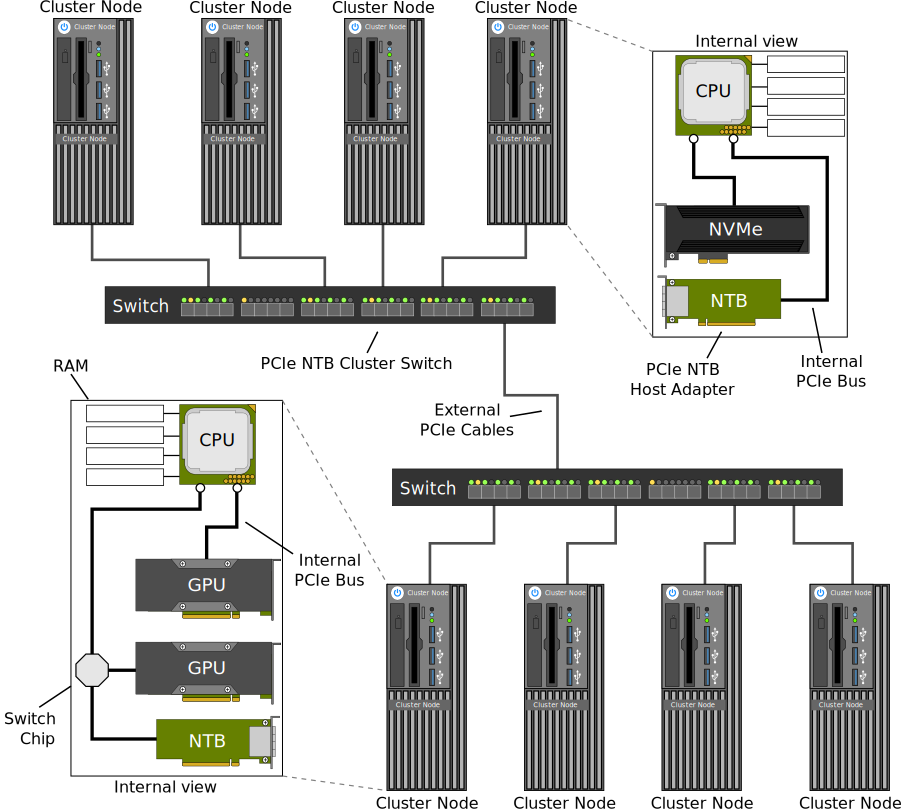
\includegraphics[width=.95\textwidth]{Cluster-Overview}
    \caption{Example of a heterogeneous \glsentrytext{pcie}-networked cluster with external cables and adapter cards capable of \glsentrytext{ntb}.}
  	\label{fig:cluster-example}
\end{figure}



%\gls{sisci}


%Traditional approaches to distributed \gls{io} over network may incur additional latency overheads
%

%However, while moving data efficiently between networked nodes in a cluster has been a research challenge for decades, moving workloads and data to remote units over the network remains a costly operation that introduces large performance overheads compared to accessing local resources. 


%Consequently, \glspl{ntb} could be exploited to create a network where the inner components of all computers in the cluster,~i.e., \glspl{cpu} and \gls{pcie} devices, are connected to the same, shared \gls{pcie} fabric.
%
    %that makes it easier for nodes to scale out in order to increase overall performance in the cluster and 
    
    %seamlessly combines distributed shared-memory functionality with traditional \gls{io}, has native \gls{pcie} performance, and simultaneously makes it easier to scale out and increase overall performance in the cluster system?

%\gls{ntb}
%\gls{pcie}
%\gls{cpu}
%\gls{fpga}
%\gls{gpu}
%\gls{dma}
%\gls{os}
%\glspl{os}
%\gls{userspace}
%\gls{sriov}

%Due to its very low latency overhead and memory addressing properties, using \gls{pcie} as a high-speed interconnection technology is a compelling alternative to traditional networking technologies. 
%
%Because \gls{pcie} was originally designed as a local \gls{io} bus, connecting devices to the \gls{cpu} on a motherboard, 
%individual computer systems operate with different \gls{pcie} address domains.
%
%Interconnecting systems using \gls{pcie} require translating memory transactions from one \gls{pcie} address domain to another. 
%
%Such address translation is made possible by using \glspl{ntb}. 
%
%By using \glspl{ntb}, a computer system can map (parts of) the address space of other, remote computer systems. 

%The \gls{ntb} translate addresses between the different address domains of the independent systems.
%

%By using \glspl{ntb}, the \gls{pcie} bus of independent computers can be interconnected, creating a network fabric where the \glspl{cpu} and internal \gls{pcie} devices of all systems are directly attached.
%%
%Through such \gls{pcie} networking, scaling out and using more hardware resources than there are available in a single computer becomes possible, increasing the overall resource utilization and system performance. 
%%
%Remote resources, such as memory and devices, could be mapped into a local system and accessed through the \gls{ntb}. 
%%
%Similarly, a remote device capable of \gls{dma} could also use the \gls{ntb} to access local resources. 
%%
%However, setting up such \gls{ntb} mappings requires awareness of the address space on the remote system.
%%
%Device drivers interacting with a remote device must use addresses that corresponds with the remote device's address space.
%%
%As this greatly increases the programming complexity and require extensive modifications to existing device driver software, it is not a viable approach for enabling resource sharing among computers  as is.



\section{Problem statement}\label{sec:objectives}
Utilizing \gls{pcie} \glspl{ntb} to share resources among machines in a \gls{pcie}-networked cluster requires a 
solution for abstracting away the physical location of a resource, including the address space of the computer system it is installed in. Moreover, as it is desirable to avoid modifications to existing device drivers and application software, such a solution must also be able to present the resource to the system as if it was locally installed.
%
Hence, the goal of this thesis is to develop an infrastructure for sharing and distributing \gls{io} resources,~i.e., devices and memory, in a way that eliminates the distinction between local and remote access of a resource. The challenges of this goal are addressed under the following research question: 
\begin{quote}\itshape
    % TODO: Consider making this more general for PCIe networks instead, and remove reference to NTBs
    %       From the objectives, it should be clear that NTBs are necessary anyway
    Can \glspl{ntb} be leveraged to allow the internal memory and devices of individual computers in a \gls{pcie}-networked cluster to be shared with and used by remote machines in the cluster, as if these resources were local to the remote machines?
\end{quote}
%
In particular, this research question can be broken down into the following objectives:
%
\begin{description}
    \item[\objective{distributed}:] Ubiquitous sharing in the cluster should be supported, allowing any machine to contribute any of its internal \gls{pcie} devices, and allowing any machine to be able to use shared devices, even contributing and using devices at the same time.
\end{description}
Perhaps the main motivation for our goal of building a system for \gls{io} resource sharing is to make it easier to scale out and use more resources than there are available in a single computer. 
If any standard \gls{pcie} device inside any machine could be shared with other machines, the \gls{io} resource utilization in the cluster can be greatly increased.
Additionally, by avoiding dedicated servers and allowing all computers in the cluster to participate in the sharing, contributing their own resources and using resources shared by others, we would effectively enable a distributed, peer-to-peer sharing model. This objective sets our goal apart from existing \gls{pcie}-based solutions, as these require a central server or that devices are directly attached to a \gls{pcie} switch.

\begin{description}
    \item[\objective{transparent}:] The fact that resources may be remote should be functionally transparent, allowing systems to use remote resources in the same way as if they were local, without requiring any modifications to device hardware, device drivers, host \gls{os}, or application software.
\end{description}
If the solution could make remote devices behave as if they were locally installed, presenting resources to the system on a level ``underneath'' the \gls{os}, it would become possible to distribute devices to \emph{physical} hosts as well, and not only \glspl{vm}. 
In other words, remote resources should appear as if they were part of the local \gls{pcie} device tree, and application software could make use of remote devices using native interfaces the same way it would use local devices.
%
Furthermore, by avoiding application- or device-specific \gls{middleware}, and instead memory-mapping remote system and device memory directly, existing device drivers and even the host \gls{os} itself would be able to interact with remote resources natively.
Avoiding any special adaptions to software would make scaling out significantly easier than what is currently possible with existing \gls{middleware}-based solutions for distributed \gls{io}, particularly those based on \gls{rdma}.

\begin{description}    
    \item[\objective{performance}:] The fact that resources may be remote should be transparent with regard to performance, remote resources should be used with native \gls{pcie} performance, and as close to local access as possible.
\end{description}
Moving data to remote units over the network introduces large performance overheads compared to accessing local resources. 
In order to further blur the hard separation between ``remote'' and ``local'', remote resources should not only behave functionally as if they were locally installed in the system using them, but also have comparable performance.
To achieve this, any communication overhead and intermediate data copying in the critical path must be completely avoided, a requirement that rules out (most) traditional methods of sharing resources over a network. 
Remote resources should be accessed directly over \emph{native} \gls{pcie}, which would improve the overall \gls{io} performance in the cluster.

\begin{description}    
    \item[\objective{dynamic}:] Shared resources should be distributed \emph{dynamically}, and direct access to device memory and system memory should be configured in run-time, also between multiple devices residing in different hosts.
\end{description}
As stated in \cref{obj:transparent}, the solution should work for physical hosts, and not only \glspl{vm}. Therefore, it must be possible to assign and reassign resources while all machines in the cluster are running, without requiring rebooting hosts or changing settings in the \gls{bios}.
For devices, this introduces the requirement that the \gls{os} supports hot-adding devices to the system --- something most modern \gls{os} implementations do.
Not only would this would allow systems to dynamically scale up or down their \gls{io} resources based on immediate workload requirements, but devices could be more efficiently partitioned between machines in the cluster, increasing the overall resource utilization. 
Furthermore, the solution should also be able to automatically discover resource location, without requiring that the user knows anything about the underlying \gls{pcie} network topology, and dynamically set up memory-mappings between devices, \glspl{cpu}, and memory resources. An example would be enabling \gls{pcie} \gls{p2p} between two or more \gls{dma}-capable devices that are physically installed in different machines.

    
\begin{description}
    \item[\objective{disaggregation}:] \Gls{disaggregation} of system memory, device memory, and device \emph{functionality} should be supported, and the solution should be able to distribute component parts to different hosts, as well as provide software facilities for resources that do not support \gls{disaggregation} in hardware.
\end{description}
Because most device drivers are written in a way that assumes exclusive control over a device, some devices implement virtualization support in hardware,~i.e., \gls{sriov}, that makes them appear to a system as having multiple \glspl{vf}. 
%
The solution should be able to \glslink{disaggregation}{disaggregate} such \gls{sriov}-capable devices, and distribute their \glspl{vf} to different machines, allowing multiple computers to use the same device simultaneously.
%
However, since not all devices implement \gls{sriov}, the solution should also provide a device driver \gls{api} that will make it possible to \glslink{disaggregation}{disaggregate} memory and device resources in software.
%
In addition to the native sharing capabilities described in \crefrange{obj:distributed}{obj:dynamic}, this \gls{api} 
would provide facilities for memory-mapping device registers as well as mapping shared memory segments for a \gls{dma}-capable device.
%
Effectively, this would bring shared-memory concepts to device driver implementations, allowing device operation and device resources to become part of the same global address space as distributed cluster applications.
%
This would allow multiple machines to simultaneously share the same, non-\gls{sriov} device, as well as making it possible to combine traditional \gls{io} with \gls{pcie} cluster capabilities such as zero-copy data transfer and multicasting.
%
Moreover, the \gls{api} should be designed so that a driver implementation does not need to consider the system-local address space of the computer system where a device is installed, thus alleviating the complexity of programming device drivers for remote devices using \glspl{ntb}.

\begin{description}    
    \item[\objective{experiments}:] To prove real-world deployment capabilities, the solution should be tested on realistic and relevant workloads and benchmarks.
\end{description}
To confirm that \gls{io} resources can be distributed to, and shared with, remote machines, a comprehensive performance evaluation covering all components of the implementation is needed.
As the solution should provide \emph{native} \gls{pcie} performance (\cref{obj:performance}), all parts should be thoroughly tested with latency and throughput in mind, in order to reveal any potential performance bottlenecks.
Standardized test suites should be used as far as possible, to prove that application software really can be unmodified (\cref{obj:transparent}).
%
Moreover, to demonstrate the completeness of the solution, the evaluation should also include workloads relying on different \gls{pcie} network topologies and include several types of devices, such as \glspl{nvme}, \glspl{gpu}, and \glspl{nic}.
%
Finally, a prototype device driver using the device driver \gls{api} (\cref{obj:disaggregation}) should be developed and evaluated. This driver should demonstrate that it is possible to \glslink{disaggregation}{disaggregate} a non-\gls{sriov} device in software, and shared with multiple machines simultaneously. The driver should also demonstrate how it can rely on memory \gls{disaggregation} and shared memory capabilities to implement data path optimizations.



\section{Scope and limitations}
% limitation: systems must support pcie p2p (or use switches that do)
%limitation: systems must support hot-plugging
%not disaggregated os, not general networks, not 50,000 nodes etc
% outside scope: orchestration, algorithms for sharing, fairness, etc
% scope
% both physical hosts and virtual hosts
% also shared memory applications
% distributed, unlike existing solutions, true peer-to-peer sharing
% commodity servers, multi platform amd, intel, arm

% performance, how much performance overhead in using remote devices?

% limitations
% safety, security (iommu, encryption)
% must use ntbs (dolphin ntbs), only sisci
% not a finished product (no orchistration sw [yet])
% for linux only?

\section{Research methodology}



\section{Contributions}
The work of this thesis contributes to the topic of \gls{io} facilitation and resource sharing in distributed computing systems, and has been presented in five peer-reviewed venues: two conference workshop publications, one short-length demonstration paper, and two journal articles.
These publications are included as \crefrange{paper:nossdav}{paper:tocs} and contain the bulk of the implementation details, particularly \cref{paper:tocs} which presents the entire solution as a whole.

We have developed a system called \emph{SmartIO} for sharing resources and distributing devices in a heterogeneous, \gls{pcie}-networked cluster.
%
In particular, the main contributions of this thesis are listed as follows:
\begin{itemize}
    \item Testing and evaluation of the \emph{Device~Lending} mechanism for \textbf{distributing \gls{pcie} devices to remote systems} (see \cref{paper:nossdav} and \cref{paper:mmsys}). Using Device~Lending, any standard \gls{pcie} device, such as \glspl{nvme}, \glspl{gpu}, \glspl{nic}, and \glspl{fpga}, may be assigned to a remote system. The device appear to the remote system as if it has been dynamically hot-added to the system, allowing existing device drivers to use the device without requiring any modifications to software.

    \item Implementation of a \textbf{new mechanism for distributing devices to \glspl{vm}} running on any host machine in the cluster (see \cref{paper:srmpds} and \cref{paper:cc}). We have developed an extension to \gls{kvm} based on the \emph{\gls{mdev}} interface, enabling direct access to remote physical hardware devices for \gls{vm} guests and setting up memory mappings for the devices. This \gls{mdev} implementation includes a method for dynamically discovering guest-physical memory layout. Using this \gls{mdev} extension, local and remote devices can be \glslink{passthrough}{``passed through''} to \glspl{vm} and used with bare-metal performance.
	
    \item Improvement of the Device~Lending and \gls{kvm}/\gls{mdev} mechanisms by implementing \textbf{support for multiple devices} and \textbf{supporting devices in different physical machines} (see \cref{paper:srmpds} and \cref{paper:cc}). A method for resolving device memory addresses and setting up memory mappings, in a way that is transparent to both the devices and the device drivers, is implemented. This enables direct data transfers between multiple devices without violating the principle of making devices appear local to the system(s) using them.

    \item Extension of the \gls{sisci} shared-memory \gls{api} with new, \textbf{device-oriented programming semantics} for writing device drivers as shared-memory applications (see \cref{paper:tocs}).
    %
	This \gls{api} extension makes it possible to \glslink{disaggregation}{disaggregate} devices and device memory in software, similarly to \gls{rdma} \gls{disaggregation} solutions.
	Unlike \gls{rdma} solutions, however, remote resources can be memory-mapped directly into the virtual address space of a software process.
	%
	Through our \gls{api} extension, device driver implementations may take full advantage of \gls{pcie} shared memory capabilities, such as remote memory access and multicasting, without requiring awareness of the underlying \gls{pcie} topology and the different address domains of remote systems.
	%
	This makes it easier to optimize data flow through the \gls{pcie} network, as software no longer needs to be written with accessing remote resources in mind, but can be implemented as if resources are local.

    \item Development of a \textbf{new prototype \gls{nvme} device driver} using our device-oriented \gls{api} extension (see \cref{paper:tocs}).\footnote{The prototype \gls{nvme} device driver is open source and can be found at \mbox{\url{https://github.com/enfiskutensykkel/ssd-gpu-dma}}}
    Although the Device~Lending mechanism and \gls{mdev} extension makes it possible to use existing device drivers, most device drivers are written in a way that assumes exclusive control over the device. Therefore, a distributed device (function) may only be used by a single user at the time.
    To demonstrate software-enabled \gls{disaggregation}, we have implemented a \emph{distributed} \gls{nvme} driver. As a proof of concept, we show a single NVMe device can be shared and operated by multiple cluster machines simultaneously, without requiring \gls{sriov}.
	This driver also demonstrates how multiple sharing aspects of SmartIO may be combined, 
	by \glslink{disaggregation}{disaggregating} remote GPU memory and enabling memory access optimizations.

    \item A \textbf{comprehensive performance evaluation} covering all parts of SmartIO and the implementation of performance optimizations (see \cref{paper:mmsys}, \cref{paper:cc}, and \cref{paper:tocs}). With the goal of not incurring any performance overhead beyond that of native \gls{pcie}, the performance of using remote resources with SmartIO is comparable to that of local access (in terms of latency and throughput).
        To prove that SmartIO is a viable and efficient solution for \gls{io} resource sharing also for realistic scenarios, two different image classification workloads relying on multiple \glspl{gpu} and \gls{nvme} storage have also been tested.
	
\end{itemize}
%
Finally, it should be noted that the research of this thesis has had impact on real systems, as several components of SmartIO have already been incorporated into the product line of Dolphin Interconnect Solutions, and others are currently being adapted for real-world deployment.\footnote{{\url{https://www.dolphinics.com/solutions/pcie_smart_io.html}}}


\section{Outline}
This thesis describes the SmartIO system for efficient sharing of resources between \gls{pcie}-networked computers.
%
The rest of this thesis is organized as follows:
\begin{description}
    \item[\cref{chapter:smartio}]
        presents the overall ideas and challenges for SmartIO. 
        We give a high-level overview of the implementation and 
        also related work

    \item[\cref{chapter:conclusion}]

    \item[\cref{paper:nossdav}]

    \item[\cref{paper:mmsys}]

    \item[\cref{paper:srmpds}]

    \item[\cref{paper:cc}]

    \item[\cref{paper:tocs}]
\end{description}


	\chapter{SmartIO}\label{chapter:smartio}
SmartIO is a solution for allowing the local resources of a machine,~i.e., memory and devices, to be shared with and used by remote machines, over standard \gls{pcie}.
%
SmartIO works for \emph{all} standard \gls{pcie} devices and their Linux device drivers, no special adaptation is needed in either hardware or software to make this sharing possible.
%
Whether devices are actually local or remote becomes irrelevant to the user, as SmartIO eliminates this distinction, with regard to both functionality and performance.
%
Furthermore, individual device functions of multi-function devices may be distributed to different machines in the network, or to the same machine should it require multiple resources.
%
It is even possible to \lgls{disaggregation}{disaggregate} a single device~(function) in software, and distribute it to multiple machines, should this be required by application software.
%
In other words, SmartIO is a solution for scaling out and using more hardware resources than there are available in a single machine.


In this chapter, we provide an overview of the SmartIO solution.
%
The complete system is described in detail in \cref{paper:tocs}.
%
\Crefrange{paper:nossdav}{paper:cc} show the evolution towards this complete system, including different iterations of individual components and parts as well as gradual performance improvements.


\section{Underlying idea}\label{sec:idea}
The defining feature of \gls{pcie} is that devices are mapped into the same address space as the \gls{cpu} and \gls{ram}.
%
This allows a \gls{cpu} to read from and write to device memory in the same manner it would access \gls{ram}.
%
Likewise, devices capable of \gls{dma} may read from and write to \gls{ram} directly.
%
\Gls{pcie} also uses \gls{msi}, allowing devices to raise interrupts by writing to an address reserved by the \gls{cpu} instead of requiring dedicated interrupt lines.


This mapping occurs when a system enumerates the \gls{pcie} bus and accesses the configuration space of each device.
%
The configuration space contains a description of the capabilities of the device, such as its memory regions.
%
The system will reserve a memory address range for each of these device memory regions.
%
By writing the start address of these regions to the device's \glspl{bar}, the device is made aware of the address space mapping.
%
Therefore, the term ``\gls{bar}'' is used synonymously for device memory regions.

%
Devices are made aware of 
The system reserves a memory address range for each of these memory regions

%introduce later: A device may even access other devices, as they too are mapped into the same address space.
However, as this mapping occurs when a \gls{cpu} enumerates the \gls{pcie} bus

By using an \gls{ntb} implementation, it is possible to connect computer systems with independent address domains together over \gls{pcie}.
%
Although not formally standardized
\begin{figure}
    \centering
    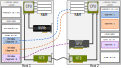
\includegraphics{ntb-example}
    \caption{test}
    \label{fig:ntb-example}
\end{figure}


\Glspl{ntb} are the most common way 

\gls{pcie}

\Glspl{ntb} are a special type ofA

\paperref{tocs}{pcie-addr}
\begin{itemize}
    \item a combined (and \textbf{shortened}!!) version of PCIe overview + NTB + mapping bars and DMA windows from previous papers
    \item simple ntb figure for mapping memory on remote node
    \item the famous device lending figure (but in a ``is this possible?'' kind of way)
    \item the general idea: can stuff (memory + bars + interrupts) be mapped through the NTB in a way that is transparent for OS?
\end{itemize}


%Unlike existing solutions for distributed \gls{io}, SmartIO seamlessly combines traditional \gls{io} with distributed shared-memory functionality, and is, therefore, able to provide sharing capabilities at multiple abstraction levels.
%Devices may be distributed to physical hosts and to \glspl{vm} alike, and SmartIO also provides facilities for \glslink{disaggregation}{disaggregating} devices and memory resources in software.


%However, as resources are accessed over native \gls{pcie}, they can be shared and used by remote machines without introducing a performance penalty.
%%
%Also unlike existing \gls{pcie}-based solutions, SmartIO is fully distributed and avoids dedicated servers.
%All machines in the cluster can contribute their own local resources and access remote resources, even at the same time.
%%
%Finally, by using \gls{pcie} shared memory techniques, SmartIO is able to abstract away the physical location of devices and memory resources. 
%Memory addresses are translated between different address domains by SmartIO in a manner that is transparent to application software, device drivers, and even the \gls{os}.
%This makes it possible to provide optimizations based on resource locality and minimizing data movement, without requiring the user to be aware of the underlying PCIe topology.
%\section{General idea}\label{sec:idea}
\section{Implementation}\label{sec:impl}
High level explanation of borrowers and lenders here.
Software architecture figure (showing the different components here)

\subsection{Device Lending}
\begin{itemize}
    \item explain shadow device
    \item intercept configuration cycles
    \item hooking DMA api for setting up DMA windows
    \item IOMMU discussion
\end{itemize}

\subsection{MDEV}
\begin{itemize}
    \item \textbf{very} brief: what is passthrough/VFIO
    \item what MDEV gives us
    \item how to map VM memory for device
    \item relaying interrupts
\end{itemize}

\subsection{API extension}
\begin{itemize}
    \item why do we need API? (disaggregation in software + shared memory networking)
    \item short explanation of SISCI
    \item what functions did we add to SISCI?
\end{itemize}

\subsection{Support for multiple lenders}
\begin{itemize}
    \item peer-to-peer device lending
    \item peer-to-peer vms
\end{itemize}


\subsection{NVMe driver}\label{sec:nvme}
\begin{itemize}
    \item why a prototype driver? demonstrate disaggregation in software
    \item why nvme? easy to parallelize because of queues
    \item driver implementation and queue sharing
    \item gpudirect + co-operation with device lending
\end{itemize}

%\section{Workload}\label{sec:eval}

\section{Performance measurements}\label{sec:eval}
Some selected performance graphs here, demonstrating zero-overhead :)

\section{Related work}\label{sec:rw}
should rw go in discussion and conclusion instead?
\begin{itemize}
    \item rdma stuff
    \item fabric partitioning: mr-iov, broadcom/microsemi chips with partitioning
    \item ladon (and other ntb stuff)
    \item disaggregation
\end{itemize}

% RW first??
%An example of this is rCUDA, where multiple clients may run jobs on the same \gls{gpu} by relying ~\cite{Duato2010}
%\Gls{rdma}-based \gls{disaggregation} can even allow a single resource to be shared by several machines in the cluster at the same time. 
%
%However, since 

	\chapter{Conclusion}\label{chapter:conclusion}
As distributed and parallel computing applications are becoming increasingly compute-intensive and data-driven, \gls{io} performance demands are ever growing.
%
Computing accelerators (such as \glspl{fpga} and \glspl{gpu}), high-throughput \glspl{nic}, and fast storage devices like \glspl{nvme}, are now commonplace in most modern computer systems.
%
For distributed computing clusters, distributing such \gls{io} resources in a way that maximizes both performance and resource utilization is a challenge.
%
In this dissertation, we have addressed this challenge and present our SmartIO framework for sharing resources between machines connected over \gls{pcie}.
%
SmartIO makes it possible to scale out and use more hardware resources than there are available in a single machine, as  machines can dynamically share their internal \gls{io} resources with other machines in a heterogeneous \gls{pcie} network.
%
Resources in remote machines can be used as if they were locally installed, without requiring any adaption to device drivers or application software and with native \gls{pcie} performance
%
Moreover, SmartIO is also able to combine traditional device \gls{io} with shared-memory capabilities, unlocking a potential by allowing devices to become part of the same global address space as distributed, cluster applications.




\section{Summary}
% - What was the target problem?
Connecting two or more independent computer systems over \gls{pcie} is possible by using \glspl{pcientb}.
%
\Glspl{ntb} have memory address translation capabilities that allow machines to map (parts of) the address space of remote systems, including \gls{ram} and device memory.
%



\glspl{ntb} to share the internal
Leveraging \glspl{ntb} to allow the internal memory and devices of individual computers to be shared with (and used by) remote machines is a challenge, as mapping remote memory resources 
%
However, in order for \glspl{ntb} to be a viable solution for sharing resources among machines connected over \gls{pcie}
% - What did you develop?


% - What were the results?



\section{Contributions}\label{sec:concl}

How did we / do this answer \crefrange{obj:distributed}{obj:experiments}?
For each objective, state clearly how it was solved and how it helps solve the overall research question as well.
%
Also, objectives should be linked to contributions list in 1.5

How does this move the world forward?


% below: how does this move the world forward
%Although many \gls{disaggregation} solutions for sharing resources over a network already exist, these solutions are often inadequate. %% compared to SmartIO
%%
%For instance, \gls{disaggregation} solutions based on \gls{rdma} introduce additional software complexity that leads to a disparity in performance, compared to a local machine using local resources. %%% compared to smartio, ....
%%
%\Gls{disaggregation} solutions based on \gls{pcie}  where the resources that can shared are limited to devices installed in dedicated servers, as these solutions lack the shared-memory capabilities necessary for sharing the inner resources of individual machines.
%

\section{Future work}\label{sec:fw}

mention new NVMe kernel space driver here

security / safety

disaggregated memory - new interconnects

iommu in tree structures is a challenge - ats? other solutions?


scaling

%Our system effectively makes all
%hosts, including their internal resources (both devices and memory), part of a common PCIe domain.


%With SmartIO, the hard separation between local and remote is blurred, as remote resources can be used as if they were locally installed and with native PCIe performance.


%Using the \gls{sisciapi}, application memory can be exported as \glspl{sharedsegment}, and \glspl{segment} in remote machines can be mapped into a local application process' virtual address space.
%By building on these concepts, our \lgls{apiext}{extension} makes it possible for a device driver implementation to use all the memory \gls{disaggregation} capabilities of \gls{sisci}, while also providing functionality for abstracting away the location of memory resources and resolving addresses between different address spaces.
%
%A device driver implemented using our \gls{apiext} can be agnostic about the underlying \gls{pcie} network topology, as devices may \gls{dma} directly to \glspl{sharedsegment}, regardless of whether they are local or remote.
%
%It is even possible to map device memory of other devices registered with SmartIO, for example devices borrowed using \gls{dl}.


	\setglossarystyle{altlist}
	\printglossary[type=main,title=\myglossarytitle]
	%\urlstyle{same} % Reset URL style for references
	\printbibliography[notkeyword=paper]
	
	% List of papers
	\paper % "Chapter" is renamed "Paper"
	%\paperpage % Similar to \part*{Papers}, but appears in TOC
	\part*{Published Papers}\addcontentsline{toc}{part}{Published Papers}
	\clearforchapter

	% Specify size of thumb indices
	\numberofpapers{5} 
    
    % Turn off listing of terms in glossaries
    \renewcommand{\lgls}[2]{%
        \glshyperlink[#2]{#1}%
    }
    \renewcommand{\gls}[1]{%
        \glshyperlink{#1}%
    }
    \renewcommand{\glspl}[1]{%
        \glshyperlink[\glsentryplural{#1}]{#1}%
    }
    \renewcommand{\glsadd}[1]{}

	\chapter{Device Lending in PCI Express Networks}
\label{paper:nossdav}
\paperthumb

\begin{description}
	\item[Authors:]
		Lars Bj{\o}rlykke Kristiansen, \textbf{Jonas Markussen}, H{\aa}kon Kvale Stensland,
		Michael Riegler, Hugo Kohmann, Friedrich Seifert, Roy Nordstr{\o}m, Carsten Griwodz, P{\aa}l Halvorsen.

	\item[Abstract:]
		The challenge of scaling \lgls{io}{IO} performance of multimedia systems to demands
		of their users has attracted much research.
		A lot of effort has gone into
		development of distributed systems that add little latency and computing overhead.
		For machines in \lgls{pcie}{PCI Express~(PCIe)} clusters,
		we propose Device Lending as a novel solution which works at a system
		level.
		%
		Device Lending achieves low latency and extremely low computing overhead without
		requiring \textit{any} application-specific distribution mechanisms.
		For the application, the remote \lgls{io}{IO} resource appears local.
		In fact, even the drivers of the operating system remain unaware that
		hardware resources are located in remote machines.
		%
		By enabling machines in a \lgls{pcie}{PCIe} cluster to lend a wide variety of hardware, 
		cluster machines can get temporary access to a pool of \lgls{io}{IO} resources. 
		Network cards, \lgls{fpga}{FPGAs}, \lgls{ssd}{SSDs}, and even \lgls{gpu}{GPUs} can easily 
		be shared among computers.
		Our proposed solution, Device Lending, works transparently without requiring any modifications to drivers,
		operating systems or software applications.

	\item[Candidate's contributions:]
		Based on Kristiansen's initial implementation of Device~Lending, Markussen had several discussions with Kristiansen and contributed to its development through testing and conducting performance benchmarks.
	    %
		Additionally, Markussen was responsible for writing most of the text and organizing the collaboration with all of the authors.
		%
		He designed and performed the performance evaluation of the Device~Lending method, and also implemented the \gls{gpu} \gls{rdma} benchmark program used in the performance evaluation.
		

	\item[Published in:]
		\emph{Proceedings of the 26th International Workshop on Network and Operating Systems Support for Digital Audio and Video}.
		NOSSDAV'16. ACM.
		May~2016, article~10, pp.~10:1--10:6.

	\item[DOI:] \href{https://doi.org/10.1145/2910642.2910650}{10.1145/2910642.2910650}

	\item[Contributed to:]
		\Cref{obj:distributed}, \cref{obj:transparent}, \cref{obj:dynamic}.

\end{description}

\includepaper{nossdav}{
	1, section, 1, Introduction, nossdav:intro,
	2, section, 1, PCI Express, nossdav:pcie,
	2, subsection, 2, Memory-mapped IO, nossdav:pcie-mmio,
	%2, subsubsection, 3, Posted and non-posted transactions, nossdav:pcie-tlp,
	%2, subsubsection, 3, Transparent bridges, nossdav:pcie-transparent,
	%2, subsubsection, 3, Non-transparent bridges, nossdav:pcie-ntb,
	%3, subsection, 2, Message-signalled interrupts, nossdav:pcie-intr,
	%3, subsection, 3, Hot-plugging, nossdav:pcie-hotplug,
	3, section, 1, Virtualization support in PCIe, nossdav:pcie-virt,
	3, subsection, 2, IO memory management unit, nossdav:pcie-iommu,
	3, subsection, 2, Single-Root IO Virtualization, nossdav:pcie-sriov,
	3, subsection, 2, Performance penalty, nossdav:pcie-iommu-performance,
	4, section, 1, Related work, nossdav:rw,
	%4, subsection, 2, Alternative protocols, nossdav:rw-rdma,
	%4, subsection, 2, Multi-Root IO Virtualization, nossdav:rw-part,
	%4, subsection, 2, Ladon and Marling, nossdav:rw-ntb,
	4, section, 1, Implementation, nossdav:impl,
	4, section, 1, Evaluation and discussion, nossdav:eval,
	5, subsection, 2, Reference evaluation, nossdav:eval-rdma,
	5, subsection, 2, Device Lending evaluation, nossdav:eval-lending,
	6, section, 1, Conclusion and future work, nossdav:concl
}

	\chapter{Efficient Processing of Videos in a Multi-auditory Environment using Device Lending of GPUs}
\label{paper:mmsys}
\paperthumb

\begin{description}
	\item[Authors:]
	Konstantin Pogorelov, Michael Riegler, \textbf{Jonas Markussen}, H{\aa}kon Kvale Stensland,
	P{\aa}l Halvorsen, Carsten Griwodz, Sigrun Losada Eskeland, Thomas de Lange.


	\item[Abstract:]
		In this paper, we present a demo that utilizes Device Lending 
		via \lgls{pcie}{PCI Express (PCIe)} in the context of a multi-auditory
		environment. Device Lending is a transparent, low-latency
		cross-machine \lgls{pcie}{PCIe} device sharing mechanism without any
		the need for implementing application-specific distribution
		mechanisms. As workload, we use a computer-aided diagnosis 
		system that is used to automatically find polyps and
		mark them for medical doctors during a colonoscopy. We
		choose this scenario because one of the main requirements
		is to perform the analysis in real-time. The demonstration
		consists of a setup of two computers that demonstrates how
		Device Lending can be used to improve performance, as well
		as its effect of providing the performance needed for 
		real-time feedback. We also present a performance evaluation
		that shows its real-time capabilities of it.


	\item[Candidate's contributions:]
		Markussen discussed and developed the idea for the paper together with Pogorelov and Riegler, where Markussen was responsible for the Device Lending setup and experiments.
		As a demonstration of a medical computational workload utilizing Device~Lending,
		Markussen performed the performance experiment together with Pogorelov.
		Markussen also contributed with text in all sections, and wrote the section on Device~Lending.

	\item[Published in:]
		\emph{Proceedings of the 7th International Conference on Multimedia Systems}. 
		MMSys'16. ACM.
		May~2016, article~36, pp.~381--386.

	\item[DOI:] \href{https://doi.org/10.1145/2910017.2910636}{10.1145/2910017.2910636}

	\item[Contributed to:]
		\Cref{obj:experiments}.

\end{description}

\includepaper{mmsys}{
	1, section, 1, Introduction, mmsys:intro,
	2, section, 1, Real-time computer aided diagnosis support, mmsys:impl,
	2, subsection, 2, GPU implementation, mmsys:impl-gpu,
	2, subsection, 2, Device Lending, mmsys:impl-lending,
	3, subsection, 2, Performance evaluation, mmsys:impl-performance,
	3, section, 1, Demonstration setup, mmsys:demo,
	4, section, 1, Conclusion and future work, mmsys:concl
}

	\include{stubs/srmpds}
	\include{stubs/cc}
	\chapter{SmartIO: Zero-overhead Device Sharing through PCIe Networking}
\label{paper:tocs}
\paperthumb

\begin{description}
	\item[Authors:]
		\textbf{Jonas Markussen}, Lars Bj{\o}rlykke Kristiansen, P{\aa}l Halvorsen,
		Halvor Kielland-Gyrud, H{\aa}kon Kvale Stensland, Carsten Griwodz.

	\item[Abstract:]
		The large variety of compute-heavy and data-driven applications accelerate the need for a distributed
		\lgls{io}{I/O} solution that enables cost-effective scaling of resources between networked hosts. For example,
		in a cluster system, different machines may have various devices available at different times, 
		but moving workloads to remote units over the network is often costly and introduce 
		large overheads compared to accessing local resources. 
		%
        To facilitate \lgls{io}{I/O} \gls{disaggregation} and device sharing among hosts connected using \lgls{pcie}{Peripheral Component Interconnect Express (PCIe)} 
		\lgls{ntb}{non-transparent bridges}, we present SmartIO. \lgls{nvme}{NVMes}, \lgls{gpu}{GPUs}, network adapters, 
		or any other standard PCIe device may be borrowed and accessed directly, as if they were local to the remote machines.
		%
		We provide capabilities beyond existing \gls{disaggregation} solutions 
		by combining traditional \lgls{io}{I/O} with distributed shared-memory functionality, allowing devices 
		to become part of the same global address space as cluster applications.
		Software is entirely removed from the data path, and simultaneous sharing of a device among 
		application processes running on remote hosts is enabled.
		%
		Our experimental results show that \lgls{io}{I/O} devices can be shared with remote hosts,
		achieving native \lgls{pcie}{PCIe} performance.
		%
		Thus, compared to existing device distribution mechanisms, SmartIO provides more efficient, low-cost resource
		sharing, increasing the overall system performance.

	\item[Candidate's contributions:]
		The ideas for the device-oriented extension to the \gls{sisci}~\gls{api} grew out from Markussen's experiences with implementing MDEV for \cref{paper:srmpds} and \cref{paper:cc}.
		%
		Markussen contributed with several new ideas for the design of this \gls{api}, and implemented these.
		%
		He collaborated on the effort of combining these ideas with previous work into the complete SmartIO system. 
		%
		Furthermore, Markussen came up with the idea for, designed, and implemented the prototype distributed \gls{nvme} driver using this \gls{api} extension, 
		including the queue offloading idea and support for running the driver on \glspl{gpu}.
		%
		Limitations in the initial \gls{api} design were uncovered during this process, and Markussen made subsequent improvements to both design and implementation of the \gls{api} throughout the development of the driver.
		%
		Additionally, he designed and implemented several workloads for this \gls{nvme} driver using \glspl{gpu} and Device~Lending
		in order to demonstrate the novelty and completeness of the SmartIO solution, as well as the performance benefits.
		%
		He conducted a thorough and exhaustive performance analysis of all components of the SmartIO system,
		as well as evaluating the entire system, and investigated and implemented solutions for eliminating performance overheads in the system.
		%
		Finally, Markussen wrote most of the text for the paper, and also wrote the necessary tools and benchmarking programs for the evaluation,
		including the \gls{fio} integration for the \gls{nvme} driver and implementing \gls{gpu} and \gls{nvme} test programs.
		

	\item[Published in:]
		\emph{Transactions on Computer Systems}. ACM.
		Published online~June~2021,
		issue~date~July~2021, 
		volume~38, issue~1-2, article~2, pp.~2:1--2:78.

	\item[DOI:] \href{https://doi.org/10.1145/3462545}{10.1145/3462545}

	\item[Contributed to:]
        All objectives (\cref{obj:distributed,obj:transparent,obj:performance,obj:dynamic,obj:disaggregation,obj:experiments}).

\end{description}

\includepaper[numbers=low][last]{tocs}{
	2, section, 1, Introduction, tocs:intro,
	5, section, 1, System overview, tocs:overview,
	6, subsection, 2, Motivation and challenges, tocs:overview-motivation,
	7, subsection, 2, Overall design, tocs:overview-design,
	9, section, 1, PCIe-interconnected clusters, tocs:pcie,
	9, subsection, 2, PCIe endpoints, tocs:pcie-ep,
	10, subsection, 2, Address-based routing, tocs:pcie-addr,
	11, subsection, 2, Non-transparent bridging, tocs:pcie-ntb,
	13, section, 1, Device Lending, tocs:lending,
	13, subsection, 2, Shadow device, tocs:lending-vdev,
	14, subsection, 2, Intercepting configuration cycles, tocs:lending-cfgspace,
	14, subsection, 2, DMA window, tocs:lending-dma,
	15, subsection, 2, Shortest path routing, tocs:lending-p2p,
	16, section, 1, VM pass-through using MDEV, tocs:mdev,
	17, subsection, 2, Mediated devices, tocs:mdev-vfio,
	18, subsection, 2, Mapping VM memory for device, tocs:mdev-dma,
	20, subsection, 2, Peer-to-peer between devices, tocs:mdev-p2p,
	20, subsection, 2, Relaying interrupts, tocs:mdev-intr,
	21, subsection, 2, VM migration, tocs:mdev-migration,
	21, section, 1, Distrubted NVMe driver, tocs:nvme,
	22, subsection, 2, Device driver API, tocs:api,
	23, subsection, 2, Driver implementation, tocs:nvme-impl,
	25, subsection, 2, Multipath failover, tocs:nvme-failover,
	26, subsection, 2, GPU support, tocs:nvme-gpu,
	29, subsection, 2, Multicast, tocs:nvme-mcast,
	29, section, 1, Performance evaluation, tocs:eval,
	31, subsection, 2, Device Lending, tocs:eval-lending,
	31, subsubsection, 3, Latency tests, tocs:eval-lending-lat,
	33, subsubsection, 3, Throughput tests, tocs:eval-lending-bw,
	35, subsubsection, 3, Longer PCIe paths, tocs:eval-lending-path,
	37, subsubsection, 3, Peer-to-peer: local vs. remote, tocs:eval-lending-p2p-1L,
	39, subsubsection, 3, Peer-to-peer: multiple lenders, tocs:eval-lending-p2p-2L,
	41, subsubsection, 3, Sharing SR-IOV devices, tocs:eval-sriov,
	45, subsection, 2, Scaling heavy workloads, tocs:eval-ml,
	46, subsection, 2, VM pass-through with MDEV, tocs:eval-mdev,
	47, subsubsection, 3, IOMMU performance penalty, tocs:eval-iommu,
	48, subsubsection, 3, Pass-through comparison, tocs:eval-mdev-vfio,
	50, subsection, 2, Distributed NVMe driver evaluation, tocs:eval-nvme,
	52, subsubsection, 3, Optimizing data access patterns, tocs:eval-nvme-sq,
	54, subsubsection, 3, Sharing a single-function NVMe device, tocs:eval-nvme-sharing,
	56, subsubsection, 3, NVMe-oF RDMA comparison, tocs:eval-nvmeof,
	60, section, 1, Discussion, tocs:disc,
	60, subsection, 2, Security, tocs:disc-security,
	61, subsection, 2, Supported OSes, tocs:disc-os,
	62, subsection, 2, Supported CPU architectures, tocs:disc-cpu,
	62, subsection, 2, Supported devices, tocs:disc-devs,
	63, subsection, 2, Alternative NTB implementations, tocs:disc-ntbs,
	63, subsection, 2, Scalability, tocs:disc-scalability,
	65, subsection, 2, Disaggregated and composable infrastructure, tocs:disc-composable,
	66, section, 1, Related work, tocs:rw,
	66, subsection, 2, PCIe fabric partitioning, tocs:rw-partitioning,
	67, subsection, 2, NTB-based solutions, tocs:rw-ntb,
	68, subsection, 2, Distributed I/O using RDMA, tocs:rw-rdma,
	70, subsection, 2, NVMe queue distribution, tocs:rw-nvme,
	70, subsection, 2, Memory disaggregation, tocs:rw-disaggr,
	72, section, 1, Conclusion, tocs:concl
}

\end{document}
